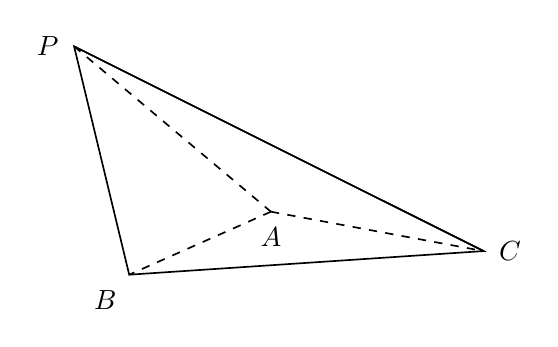
\begin{tikzpicture}[line width=0.6pt, font=\normalsize]
\coordinate (P) at (-2.4,1.9);
\coordinate (B) at (-1.7,-1.0);
\coordinate (C) at (2.8,-0.7);
\coordinate (A) at (0.1,-0.2);
\draw[draw=black] (P) -- (B) -- (C) -- cycle;
\draw[draw=black] (P) -- (C);
\draw[draw=black,dashed] (P) -- (A);
\draw[draw=black,dashed] (A) -- (B);
\draw[draw=black,dashed] (A) -- (C);
\node[left,xshift=-2pt] at (P) {$P$};
\node[below left,xshift=-1pt,yshift=-2pt] at (B) {$B$};
\node[right,xshift=2pt] at (C) {$C$};
\node[below,yshift=-2pt] at (A) {$A$};
\end{tikzpicture}
